\jxhj{%教学后记
	}
\skrq{%授课日期
	2018年1月16日 4-5节}
\ktmq{%课题名称
	 期末复习}
\jxmb{%教学目标,每行前面要加 \item
	\item 掌握中级工考证的编程技巧;
	\item 提高编程速度;
	\item 复习本学期所学知识。
}
\jxzd{%教学重点,每行前面要加 \item
	\item 中级工考证的编程技巧;
	\item 复习本学期所学知识。 }
\jxnd{%教学难点,每行前面要加 \item
	\item 提高编程速度。 }
\jjff{%教学方法
	通过讲述、举例、演示法来说明;}

\makeshouye %制作教案首页

%%%%教学内容
\subsection{组织教学}
\begin{enumerate}[\hspace{2em}1、]
	\item 集中学生注意力;
	\item 清查学生人数;
	\item 维持课堂纪律;
\end{enumerate}

\subsection{复习导入及主要内容}
\begin{enumerate}[1、]
\item Z向分层;
\item IF Then 指令;
\item Z向分层的应用;
\item 多个循环的应用。
\end{enumerate}

\subsection{教学内容及过程}
	
\subsubsection{小结}
	本学期教学工作上的总结,学生学习上的总结,学生作业完成上的总结,学生实习操作上的总结,学生实习报告上的总结,及总体评介,肯定其优点,并指出不足。

\subsubsection{期终考试相关知识}
	选择、判断、填空、问答、编程、作图、改错。
\subsubsection{复习基本指令}

	G指令

	G0 G1 G2 G3

	G17 G18 G19

	G9 G61 G62 G63 G64

	G4 

	G20 G21

	G40 G41 G42 

	G43 G44 G49

	G90 G91

	G98 G99

	G81 G82 G83 G84 G85 G86 G87 G88 G89 G80 G73 G74 G76

	M指令

	M0 M1 M2 M30

	M3 M4 M5 M19

	M6 M7 M8 M9

	M98 M99

	其它指令

\subsubsection{复习相关知识}

	数控加工工艺学

	数学知识

	刀具、量具的选择及使用

	热处理、

	计算机知识

	CAD/CAM

\subsubsection{复习机床操作知识}

	操作方式:回零、手动、手轮、MDI、自动、快速、编辑

	开机

	手动回参考点

	手动返回

	输入程序

	参数设定

	程序检查及测试

	自动加工

	测量

	安全

\subsubsection{复习编程思路}

	平面

	外轮廓

	挖槽(岛屿)

	孔、

	凸轮槽

	薄壁

	复杂零件

	配合零件

	CAD/CAM

	宏程序

\begin{figure}[h]
	\centering
	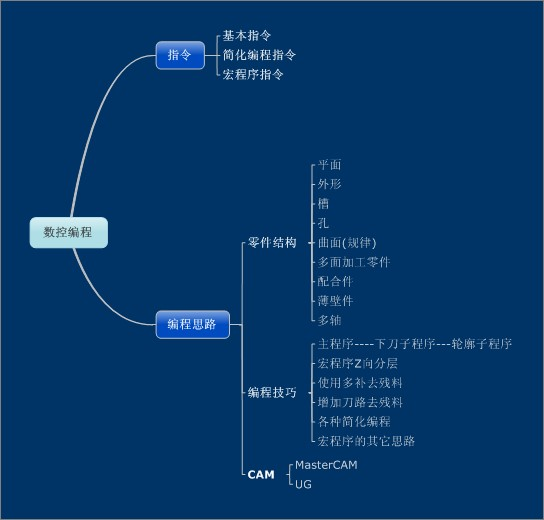
\includegraphics[width=0.9\linewidth,trim=0 0 0 0,clip]{data/image/35-1}
	\caption{复习}
	\label{fig:35-1}
\end{figure}

\subsection{课堂小结}
\begin{enumerate}[1、]
\item Z向分层;
\item IF Then 指令;
\item Z向分层的应用;
\item 多个循环的应用。
\end{enumerate}

\vfill
\subsection{布置作业}
\begin{enumerate}[1、]
	\item 综合习题一。
\end{enumerate}
\vfill